% $Id: ESMF_infradataoverview.tex,v 1.18 2004/05/17 22:25:55 jwolfe Exp $

\section{Overview of Infrastructure Data Handling}

The ESMF infrastructure data classes are part of the framework's 
hierarchy of structures for handling Earth system model data and 
metadata on parallel platforms.  The hierarchy is in complexity; the 
simplest data class in the infrastructure represents a distributed 
array and the most complex data class represents a bundle of physical 
fields that are discretized on the same grid.  Data class methods 
are called both from user-written code and from other classes 
internal to the framework. 

Data classes are distributed over {\bf DE}s, or {\bf Decomposition Elements}.  
A DE represents a piece of a decomposition.  A DELayout is a collection
of DEs with some associated connectivity that describes a specific 
distribution.  For example, the distribution of a grid divided 
into four segments in the x-dimension would be expressed in ESMF as
a DELayout with four DEs lying along an x-axis. This abstract concept 
enables a data decomposition to be defined in 
terms of threads, MPI processes, virtual decomposition elements, or
combinations of these without changes to user code.  This is a
primary strategy for ensuring optimal performance and portability
for codes using the ESMF for communications.

ESMF data classes are useful because they provide a standard, 
convenient way for developers to collect together information 
related to model or observational data.  The information assembled 
in a data class includes a data pointer, a set of attributes 
(e.g. units, although attributes can also be user-defined), and a 
description of an associated grid.  The same set of information within 
an ESMF data object can be used by the framework to arrange 
intercomponent data transfers, to perform I/O, for communications
such as gathers and scatters, for simplification of interfaces 
within user code, for debugging, and for other functions.  
This unifies and organizes codes overall so that the user need not
define different representations of metadata for the same field 
for I/O and for component coupling.  

Since it is critical that users be able to introduce ESMF into their
codes easily and incrementally, ESMF data classes can be created based 
on native Fortran pointers.  Likewise, there are methods for retrieving 
native Fortran pointers from within ESMF data objects.  This allows
the user to perform allocations using ESMF, and to retrieve Fortran
arrays later for optimized model calculations.  The ESMF data classes 
do not have associated differential operators or other mathematical 
methods.

For flexibility, it is not necessary to build an ESMF data object 
all at once.  For example, it's possible to create a 
field but to defer allocation of the associated field data until 
a later time.


\begin{center}  
\begin{tabular}{|p{6in}|}
\hline
\vspace{.01in}
{\bf Key Features} \\[.01in]
Hierarchy of data structures designed specifically for the Earth 
system domain and high performance, parallel computing. \\
Multi-use ESMF structures simplify user code overall. \\
Data objects support incremental construction and deferred allocation. \\ 
Native Fortran arrays can be associated with or retrieved from ESMF data
objects, for ease of adoption, convenience, and performance. \\[.03in] \hline
\end{tabular}
\end{center}

\subsection{Infrastructure Data Classes}

The main classes that are used for model and observational data manipulation
are as follows:

\begin{itemize}

\item {\bf Array}  An ESMF Array contains a data pointer, 
information about its associated datatype, precision, and 
dimension.  

Data elements in Arrays are partitioned into categories 
defined by the role the data element plays in distributed halo 
operations.  Haloing - sometimes called ghosting - is the 
practice of copying portions of array data to multiple memory 
locations to ensure that data dependencies can be satisfied 
quickly when performing a calculation.  ESMF Arrays contain 
an {\bf exclusive} domain, which contains data elements
updated exclusively and definitively by a given DE; a 
{\bf computational} domain, which contains all data elements
with values that are updated by the DE in computations; and 
a {\bf total} domain, which includes both the computational 
domain and data elements from other DEs which may be read 
but are not updated in computations.

\item {\bf Field}  A Field holds model and/or observational 
data together with its underlying grid or set of spatial 
locations.  It provides methods for configuration, 
initialization, setting and retrieving data values, 
data I/O, data regridding, and manipulation of attributes.

\item {\bf Bundle} Groups of Fields on the same underlying 
physical grid can be collected into a single object called a Bundle.  
A Bundle provides two major functions: it allows groups of 
Fields to be manipulated using a single identifier, for example 
during export or import of data between Components; and 
it allows data from multiple Fields to be packed together 
in memory for higher locality of reference and ease in 
subsetting operations.  Packing a set of Fields into a single
Bundle before performing a data communication allows the set 
to be transferred at once rather than as a Field at a time.
This can improve performance on high-latency platforms.

Bundle objects contain methods for setting and retrieving constituent 
fields, regridding, data I/O, and reordering of data in memory.

\end{itemize}

\subsection{Object Model}

The following is a simplified UML diagram showing the relationships among
ESMF Field, Grid and Bundle classes.  See Appendix A, {\it A Brief 
Introduction to UML},
for a translation table that lists the symbols in the diagram and their 
meaning.

\begin{center}
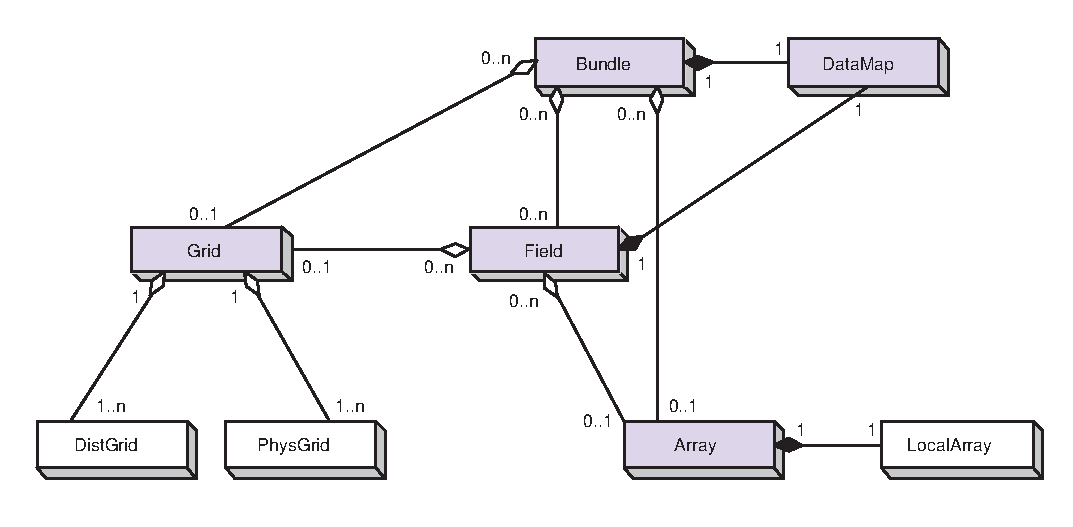
\includegraphics{Bundle_obj.eps}   
\end{center}










